\clearpage
\newpage
\section{Auswertung}
	\label{sec:auswertung}

	Um die dynamische Viskosit"at zu bestimmen, m"ussen vorab verschiedene Messungen durchgef"uhrt werden.
	Zun"achst sollen daf"ur die Gr"o"sen $K$ der Gleichung \eqref{viskositaet_0} und sp"ater die Konstanten $A$ und $B$ der Gleichung \eqref{viskositaet_dyn} ermittelt werden.
	Schlie"slich wird "uberpr"uft, ob die untersuchte Str"omung tats"achlich laminar ist.

	\subsection{Bestimmung der Apparaturkonstante $K$} % (fold)
		\label{sub:bestimmung_k}

		Es stehen zwei unterschiedlich gro"se Kugeln zur Verf"ugung, die das Viskositmeter pas\-sie\-ren k"onnen.
		Die Konstante $K_\mathrm{klein}$ ist f"ur die kleinere Kugel gegeben, wodurch zun"achst die Viskosit"at $\eta_0$ bei Raumtemperatur ($T = \SI{20}{\celsius}$) bestimmt werden kann.
		Mit Kenntnis dieser Gr"o"se l"asst sich anschlie"send die entsprechende Konstante $K_\mathrm{gro"s}$ f"ur die sp"ater ver\-wen\-de\-te gro"se Kugel bestimmen.

		Es werden zehn Messwerte f"ur die Fallzeit $t$ der kleinen Kugel aufgenommen:

		\begin{table}[h!]
			\centering
			\caption{Messwerte der Fallzeit $t$ der kleinen Kugel bei Raumtemperatur}
			\begin{tabular}{|c|c||c|c|}
				\hline
				Messung & $t [\mathrm{s}]$ & Messung & $t [\mathrm{s}]$ \\
				\hline
				\hline
				1	&	12.92 &	6	&	12.86 \\
2	&	12.81 &	7	&	12.84 \\
3	&	12.87 &	8	&	12.84 \\
4	&	12.52 &	9	&	12.73 \\
5	&	12.78 &	10	&	12.60 \\
				\hline
			\end{tabular}
		\end{table}

		Es wird ein Mittelwert mit mittlerem Fehler gebildet:

		\begin{equation*}
			t_\mathrm{klein} = \SI{12.78 (04)}{\second} .
		\end{equation*}

		Desweiteren muss aus dem Durchmesser $d_\mathrm{klein}$ und der Masse $m_\mathrm{klein}$ die Dichte $\rho_{K,\mathrm{klein}}$ der Kugel bestimmt werden. Es gilt

		\begin{equation*}
			\rho = \frac{m}{V} = \frac{6 m}{\pi d^3} .
		\end{equation*}

		Die Masse ist hierbei bekannt, der Durchmesser muss mit einem Messschieber gemessen werden, wobei der Ablesefehler $\Delta d = \SI{.05}{\milli \meter}$ betr"agt.

		Durch Gau"s'sche Fehlerfortpflanzung erh"alt man einen Fehler 
		\begin{equation*}
			\Delta \rho = \left| \frac{\partial \rho}{\partial d} \right| \cdot \Delta d = \frac{18m}{\pi d^4} \cdot \Delta d .
		\end{equation*}

		Damit kann die Dichte bestimmt werden:

		\begin{eqnarray*}
			d_\mathrm{klein} & = & \SI{15.64 (5)}{\milli \meter} \\ 
			m_\mathrm{klein} & = & \SI{4.4531}{\gram} \\
			\Rightarrow \quad \rho_\mathrm{klein} & = & \SI{2.223 (21)}{\gram \per \centi \meter \cubed} .
		\end{eqnarray*}

		Mit den obigen Gr"o"sen wird $\eta_0$ bestimmt.
		Auch hier erh"alt man einen Fehler durch Fehlerfortpflanzung:

		\begin{equation*}
			\Delta \eta = \left| \frac{\partial \eta}{\partial \rho_K} \right| \cdot \Delta \rho_K + \left| \frac{\partial \eta}{\partial t} \right| \cdot \Delta t = K \left(t \cdot \Delta \rho_K + \left|\rho_K - \rho_\mathrm{Fl}\right| \cdot \Delta t \right)
		\end{equation*}

		Die Dichte $\rho_\mathrm{Fl}$ des Wassers und die Konstante $K_\mathrm{klein}$ sind bekannt \cite{uni_magdeburg} \cite{anleitung} . Man erh"alt

		\begin{eqnarray*}
			K_\mathrm{klein} & = & \SI{.0764}{\milli \pascal \centi \meter \cubed \per \gram} \\
			\rho_\mathrm{Fl} & = & \SI{.998}{\gram \per \centi \meter \cubed}\\
			\Rightarrow \quad \eta_0 & = & \SI{1.196 (6)}{\kilo \gram \per \meter \per \second} .
		\end{eqnarray*}

		Nun kann $K_\mathrm{gro"s}$ der gro"sen Kugel bestimmt werden.
		Hierf"ur werden die gleichen Messungen mit der zweiten Kugel wiederholt.

		\begin{table}[h!]
			\centering
			\caption{Messwerte der Fallzeit $t$ der gro"sen Kugel bei Raumtemperatur}
			\begin{tabular}{|c|c||c|c|}
				\hline
				Messung & $t [\mathrm{s}]$ & Messung & $t [\mathrm{s}]$ \\
				\hline
				\hline
				1	&	94.89 &	6	&	95.44 \\
2	&	95.35 &	7	&	95.46 \\
3	&	95.15 &	8	&	95.29 \\
4	&	95.64 &	9	&	95.40 \\
5	&	94.20 &	10	&	95.37 \\
				\hline
			\end{tabular}
		\end{table}

		\begin{equation*}
			\overline{t} = \SI{95.22 (13)}{\second}
		\end{equation*}

		Masse $m$ und Durchmesser $d$ dieser Kugel werden gemessen und Dichte $\rho$ bestimmt. Die Ablesefehler betragen $\Delta m = \SI{.05}{\gram}$ und $\Delta d = \SI{.05}{\milli \meter}$.
		Weil nun auch $m$ fehlerbehaftet ist erh"alt man

		\begin{equation*}
			\Delta \rho = \frac{6}{\pi d^3} \left( \frac{3 m}{d} \cdot \Delta d + \Delta m \right)
		\end{equation*}

		\begin{eqnarray*}
				m & = & \SI{4.60 (5)}{\gram} , \\
				d & = & \SI{15.82 (5)}{\milli \meter} , \\
				\Rightarrow \quad \rho & = & \SI{2.219 (45)}{\gram \per \centi \meter \cubed}
		\end{eqnarray*}

		Durch Umstellen der Gleichung \eqref{viskositaet_0} erhalten wir

		\begin{equation}
			K = \frac{\eta}{\left(\rho_K - \rho_\mathrm{Fl}\right) \overline{t}} .
		\end{equation}

		Mit Gau"s'scher Fehlerfortpflanzung erh"alt man dann den Fehler

		\begin{equation*}
			\Delta K = \frac{\Delta \eta}{\left|\rho_K - \rho_\mathrm{Fl}\right| t} + \frac{\eta}{\left|\rho_K - \rho_\mathrm{Fl}\right| t} \left[ \frac{\Delta \rho_K}{\left| \rho_K - \rho_\mathrm{Fl} \right|} + \frac{\Delta t}{t} \right] .
		\end{equation*}

		\begin{equation*}
			\Rightarrow \quad K = \SI{10.28 (44)}{\milli \pascal \centi \meter \cubed \per \gram}
		\end{equation*}

	\subsection{Temperaturabh"angigkeit der Viskosit"at $\eta$ von destilliertem Wasser}
		\label{sub:temperaturabhaengigkeit}

		Da nun $K_\mathrm{gro"s}$ bekannt ist, kann die dynamische Viskosit"at $\eta (T)$ f"ur verschiedene Tem\-pe\-ra\-tu\-ren $T$ mit Messung der Fallzeit $t$ bestimmt werden.
		Durch eine lineare Regression der Werte $\ln{\eta (T)}$ und $1 / T$ lassen sich die Konstanten $A$ und $B$ aus Gleichung \eqref{viskositaet_dyn} bestimmen.

		Zu jeder Temperatur werden zwei Messwerte aufgenommen. Die folgende Tabelle zeigt die Messwerte

		\begin{table}[h!]
			\centering
			\caption{Mittelwerte der Fallzeit $\overline{t}$ der gro"sen Kugel in Abh"angigkeit der Temperatur $T$}
			\begin{tabular}{|c|c||c|c|}
				\hline
				$T [\SI{}{\celsius}]$ & $t [\mathrm{s}]$ & $T [\SI{}{\celsius}]$ & $t [\mathrm{s}]$ \\
				\hline
				\hline
				27	&	82.58	&	42	&	61.73 \\
27	&	82.43	&	42	&	61.80 \\
30	&	79.09	&	45	&	58.40 \\
30	&	79.23	&	45	&	58.33 \\
33	&	73.46	&	48	&	55.40 \\
33	&	73.52	&	48	&	54.32 \\
36	&	69.81	&	51	&	52.80 \\
36	&	69.61	&	51	&	53.03 \\
39	&	64.86	&	54	&	50.78 \\
39	&	65.16	&	54	&	50.35 \\
				\hline
			\end{tabular}
		\end{table}

		Aus jedem Wert kann nun mit Gleichung \eqref{viskositaet_dyn} die Viskosit"at $\eta (T)$ bestimmt werden.
		Die oben beschriebene lineare Regression durch numpy liefert dann

		\begin{eqnarray*}
			A & = & \SI{.396 (28)}{\kilo \gram \per \meter \per \second} \\
			B & = & \SI{27.37 (107)}{\second} .
		\end{eqnarray*}

		\begin{figure}[h!]
			\centering
			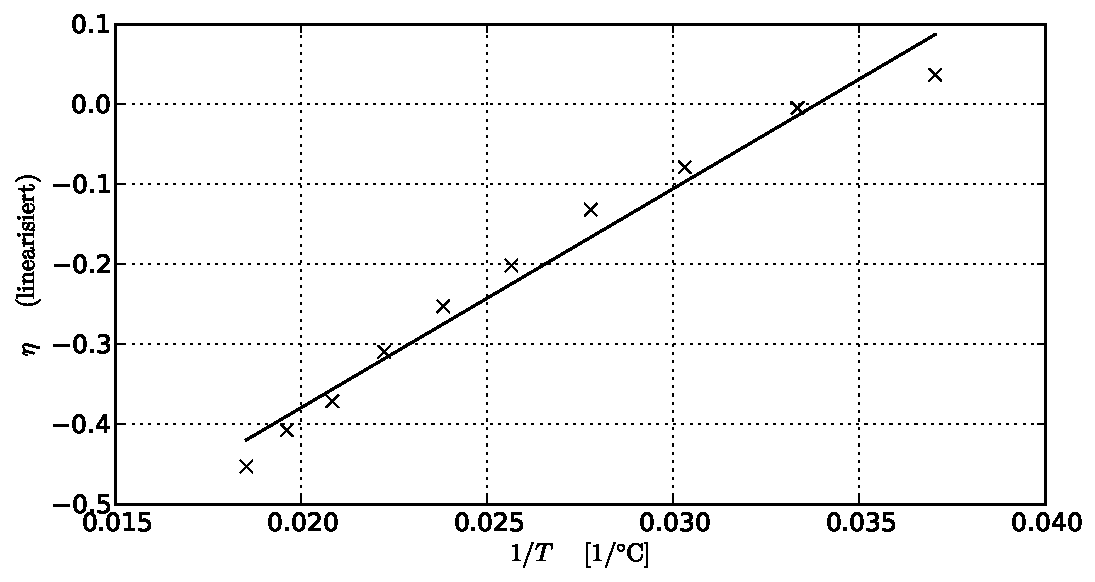
\includegraphics[width = 15cm]{img/plot.pdf}
			\caption{Werte und Ausgleichsgerade der linearen Regression f"ur $\ln{\eta}$ und $1 / T$}
			\label{fig:regression}
		\end{figure}

		\begin{figure}[h!]
			\centering
			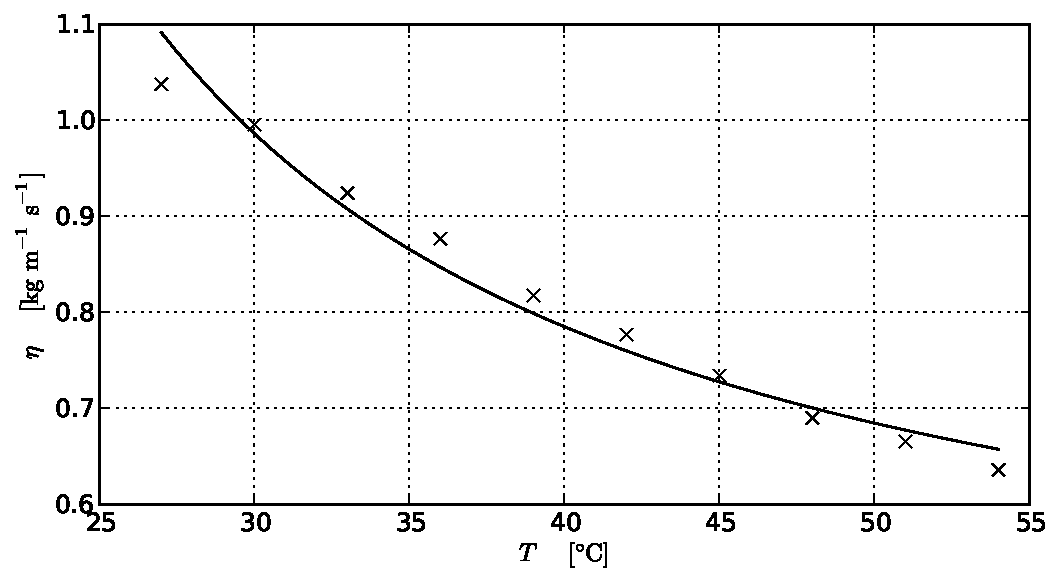
\includegraphics[width = 15cm]{img/plot2.pdf}
			\caption{Werte und Theoriekurve f"ur $\eta(T)$ und $T$}
			\label{fig:graph}
		\end{figure}

	\clearpage

	\subsection{"Uberpr"ufung auf laminare Str"omung}
		\label{sub:laminar}

		Schlie"slich wird "uberpr"uft, ob die vorliegende Str"omung laminar ist -- ob also keine Turbulenzen im Wasser auftreten.
		Dazu muss die Reynoldszahl $Re$ deutlich unter $Re_\mathrm{krit} = 2050$ liegen.
		Der Wert berechnet sich nach

		\begin{equation*}
			Re = \frac{\rho v d_\mathrm{B}}{\eta} ,
		\end{equation*}

		wobei $v$ die charakteristische Str"omungsgeschwindigkeit der Fl"ussigkeit gegen"uber dem K"orper und $d$ die Bezugsl"ange bezeichnet.

		Es wird der maximale Wert $Re_\mathrm{max}$ ermittelt, der in diesem Versuch erreicht wird.
		Mit einer Gef"a"sl"ange von $x = \SI{10}{\centi \meter}$ erh"alt man die Geschwindigkeit $v_\mathrm{max}$, f"ur die die Reynoldszahl maximal wird.
		Au"serdem w"ahlt man aus den Messwerten die Viskosit"at $\eta_\mathrm{max}$, f"ur welche dies ebenfalls gilt.
		Die Bezugsl"ange $d_\mathrm{B}$ entspricht hierbei dem Durch\-messer der Kugel ($d_\mathrm{B} = d$).
		Gau"s'sche Fehlerfortpflanzung liefert

		\begin{eqnarray*}
			\Delta Re & = & \frac{\rho}{\eta} \left( d \Delta v + v \Delta d + \frac{v d}{\eta} \Delta \eta \right) , \\
			\Delta v & = & \frac{x}{t^2} \Delta t.
		\end{eqnarray*}

		Dann folgt:

		\begin{eqnarray*}
			v_\mathrm{max} & = & \frac{\SI{10}{\centi \meter}}{\SI{50.565}{\second}} = \SI{.198}{\centi \meter \per \second} , \\
			\eta_\mathrm{max} & = & \SI{6.36}{\gram \per \centi \meter \per \second} , \\
			d & = & \SI{1.582}{\centi \meter} \\
			\Rightarrow \quad Re & = & \SI{.049}{} \ll Re_\mathrm{krit} .
		\end{eqnarray*}

		Somit liegt hier eine laminare Str"omung vor.
		Die Messfehler wurden dabei nicht be\-trach\-tet, weil sie einige Gr"o"senordnungen kleiner sind als der Wert der Reynoldszahl.
